\begin{figure}[htbp]
	\centering
	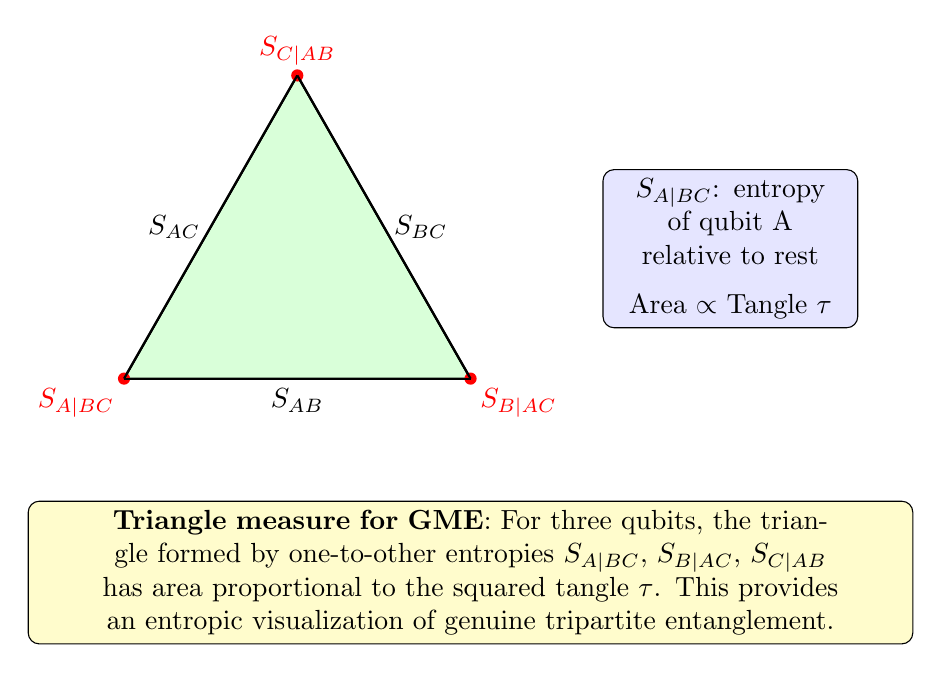
\begin{tikzpicture}[scale=1.1]
		\coordinate (A) at (-2,0);
		\coordinate (B) at (2,0);
		\coordinate (C) at (0,3.5);

		\draw[thick, fill=green!15] (A) -- (B) -- (C) -- cycle;

		\fill[red] (A) circle (2pt) node[below left] {$S_{A|BC}$};
		\fill[red] (B) circle (2pt) node[below right] {$S_{B|AC}$};
		\fill[red] (C) circle (2pt) node[above] {$S_{C|AB}$};

		\draw[thick] (A) -- (B) node[midway, below] {$S_{AB}$};
		\draw[thick] (B) -- (C) node[midway, right] {$S_{BC}$};
		\draw[thick] (C) -- (A) node[midway, left] {$S_{AC}$};

		\node[draw, rounded corners, fill=blue!10, text width=3cm, align=center] at (5,1.5) {
			$S_{A|BC}$: entropy of qubit A relative to rest\\
			\vspace{0.2cm}
			Area $\propto$ Tangle $\tau$
		};

		\node[draw, rounded corners, fill=yellow!20, text width=11cm, align=center, below=1cm] at (2,-0.5) {
			\textbf{Triangle measure for GME}: For three qubits, the triangle formed by one-to-other entropies $S_{A|BC}$, $S_{B|AC}$, $S_{C|AB}$ has area proportional to the squared tangle $\tau$. This provides an entropic visualization of genuine tripartite entanglement.
		};
	\end{tikzpicture}
	\caption{Triangle measure for three-qubit genuine multipartite entanglement. The one-to-other entropies $S_{A|BC}$, $S_{B|AC}$, $S_{C|AB}$ form a triangle whose area is proportional to the squared tangle $\tau$. This connects geometric and entropic measures of entanglement.}
	\label{fig:triangle-measure}
\end{figure}
